%%%%%%%%%%%%%%%%%%%%%%%%%%%%%%%%%%%%%%%%%%%%%%%%%%%%%%%%%%%%%%%%%%%%%%%%%%%%%%%%
\chapter{Introduction}\label{chap:intro}
%%%%%%%%%%%%%%%%%%%%%%%%%%%%%%%%%%%%%%%%%%%%%%%%%%%%%%%%%%%%%%%%%%%%%%%%%%%%%%%%
The recovery of the underlying structure of a scene captured in an image is 
arguably one the core problems in Computer Vision. Although many properties
of a scene may be recovered, it is the geometry of the objects within the scene
that is of most use in many problems, as the geometry provides a strong model
from which to perform inference. In particular, the 3D shape of the underlying
objects is arguably the strongest cue for common tasks such as object
recognition and object localisation. However, the general problem or recovering
the 3D shape of an object from image (s) is incredibly ill-conditioned. Even when 
provided with multiple images, or additional information about the scene or
capturing conditions, 3D recovery is rife with ambiguities. As demonstrated
by~\cref{tbl:3d_recovery_methods}, many strategies have been proposed for
solving this problem.

In contrast to the difficulty of the general case, the recovery of 3D facial
has been highly successful. Human faces have a number of qualities that are
highly desirable for shape recovery: they are extremely homogenous in
configuration (all healthy human faces have two eyes, a nose and mouth in the 
same approximate location), convex, exhibit approximately lambertian 
reflectance~\cite{Sirovich:1987te,RefWorks:314,Basri:2003ie,RefWorks:98,Hallinan:1994dz},
are largely captured from a single direction (frontal) and are deformable
but not self occluding. Furthermore, there exists a large amount of publicly
available imagery of faces and human faces are of significant interest to a 
number of fields including entertainment, medicine and psychology.
%%%%%%%%%%%%%%%%%%%%%%%%%%%%%%%%%%%%%%%%
\begin{table}[t]
	\centering
	\resizebox{\textwidth}{!}{%
		\begin{tabular}{@{}llccl@{}}
		\toprule
		\multicolumn{1}{c}{Classification}                  & \multicolumn{1}{c}{Method}                                                   & \# Images & Other Input                                                                       & \multicolumn{1}{c}{Output} \\ \midrule
		\multirow{4}{*}[-0.7cm]{Image Formation}            & Shape-from-Shading                                                           & $1$       & \begin{tabular}[c]{@{}c@{}}Reflectance Model, \\ Lighting Directions\end{tabular} & Surface Normals            \\ \cmidrule(l){3-5} 
		                                                    & \begin{tabular}[c]{@{}l@{}} (Un) Calibrated \\ Photometric Stereo\end{tabular} & $\geq 3$  & \begin{tabular}[c]{@{}c@{}}Lighting Directions \\ (If Calibrated)\end{tabular}    & Surface Normals            \\ \cmidrule(l){3-5} 
		                                                    & Shape-from-Contour                                                           & $1$       & Object Contour                                                                    & Coarse Surface Normals     \\ \cmidrule(l){3-5} 
		                                                    & Analysis-by-Synthesis                                                        & $1$       & 3D Model                                                                          & 3D Shape                   \\ \midrule
		\multicolumn{1}{c}{\multirow{2}{*}{Photogrammetry}} & Multi-View Stereo                                                            & $k$       & Camera Extrinsics                                                                 & 3D Shape                   \\ \cmidrule(l){3-5} 
		\multicolumn{1}{c}{}                                & Structure-from-Motion                                                        & $k$       & Corresponding Points                                                              & 3D Shape                   \\ \midrule
		\multicolumn{1}{c}{Other}                           & Shape Transfer                                                               & $1$       & 3D Model                                                                          & 3D or 2.5D Shape           \\ \bottomrule
		\end{tabular}
	}
	\caption{A summary of methods for recovering 3D shape from images. The two 
	         largest subcategories are image formation algorithms and 
	         photogrammetry.}
\label{tbl:3d_recovery_methods}
\end{table}
%%%%%%%%%%%%%%%%%%%%%%%%%%%%%%%%%%%%%%%%
An impressive example of the quality of 3D reconstruction possible is he seminal 
work of Blanz and Vetter~\cite{RefWorks:96}. A commercial example of the 
quality of reconstruction provided by a 3D Morphable Model (3DMM) method
is given in~\cref{fig:facegen_tom_hanks}. However, despite the success of 
3DMMs~\cite{RefWorks:96}, the problem of high quality 3D facial 
surface recovery from challenging images is still far from solved. For example,
the recovery of 3D facial surfaces under arbitrary conditions,
so called ``in-the-wild'' images, remains a challenging and active area of
research~\cite{KemelmacherShlizerman:2013iv,Suwajanakorn:2015gf,Suwajanakorn:2014bl,Snape:2015gl,Roth:2015hq}.
In the case of 3DMMs, ``in-the-wild'' images present a significant challenge
as 3DMMs attempt to recover shape via an ``analysis-by-synthesis'' approach. An
``analysis-by-synthesis'' approach involves attempting to minimise the 
reconstruction error between the input image and a rendered output image that
is modelled via a set of parametric models and lighting conditions. Therefore,
in the case of ``in-the-wild'' facial images, ``analysis-by-synthesis'' is
incredibly challenging as an accurate result would require photorealistic
rendering, which is currently not possible within the Computer Vision
literature. Moreover, the parametric models employed are necessarily low-rank
and therefore are not able to model fine details such as wrinkles.

% Need to mention about alignment

In this thesis, I am interested in tackling the problem of 3D facial shape
recovery from challenging ``in-the-wild'' conditions. This is in contrast
to many works, such as the 3DMM, that focus on the recovery of facial shape
under ideal conditions (uniform frontal illumination, frontal face,
no expression, young caucasian subject). As previously mentioned and summarised
in \cref{tbl:3d_recovery_methods}, there are 
a number of scenarios that may be considered in order to recover shape from
images. Given the breadth of possible scenarios, I have categorised them into
three major areas:
%%%%%%%%%%%%%%%%%%%%%%%%%%%%%%%%%%%%%%%%
\begin{itemize}
	\item \textbf{Single Image.} Given a single image, estimate the facial 
	      shape. This may involve employing template facial shapes, parametric
	      facial models or knowledge of the lighting conditions. 
	\item \textbf{Image Collections.} Given multiple images of faces, that may
	      or may not be of the same individual, estimate the facial shape for
	      each image. This may involve parametric models, employing illumination
	      constraints or known correspondances between the images.
	\item \textbf{Videos.} Given a sequence of images of a single individual,
	      recover their facial shape. This may involve known correspondances or
	      parametric models.
\end{itemize}
%%%%%%%%%%%%%%%%%%%%%%%%%%%%%%%%%%%%%%%%
Although there may be many more possible scenarios than those described above, 
these three scenarios are very common representations of the type of media 
available for faces. In this thesis, I chose to investigate a novel method
of improving the state-of-the-art under each of these three scenarios.
%%%%%%%%%%%%%%%%%%%%%%%%%%%%%%%%%%%%%%%%
\begin{figure}[t]
	\centering
	\hspace*{\fill}
	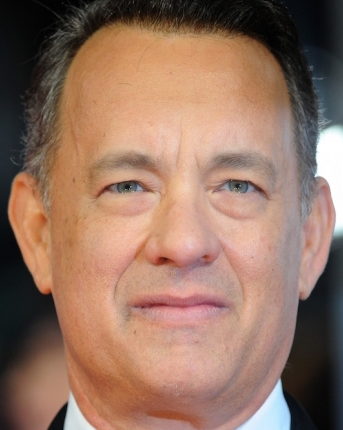
\includegraphics[height=1.8in]{introduction/images/tom_hanks_frontal_awards}\hfill
	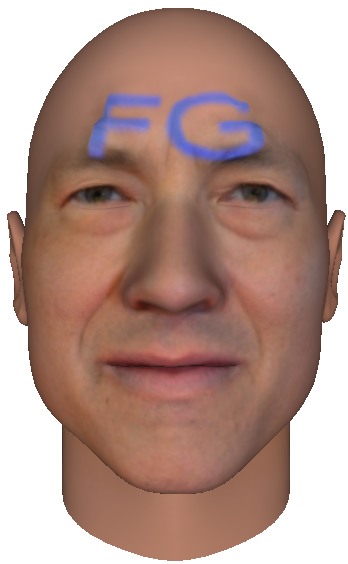
\includegraphics[height=1.8in]{introduction/images/tom_hanks_frontal_awards_facegen}\hfill
	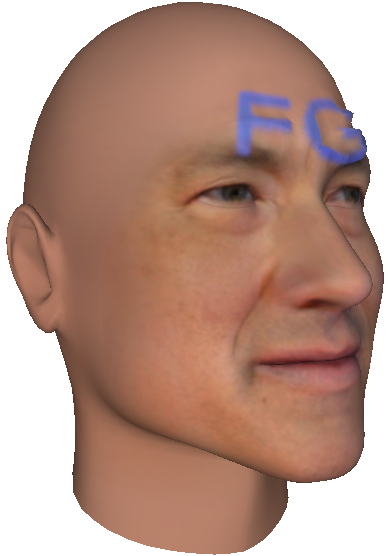
\includegraphics[height=1.8in]{introduction/images/tom_hanks_frontal_awards_facegen_profile}\hfill
	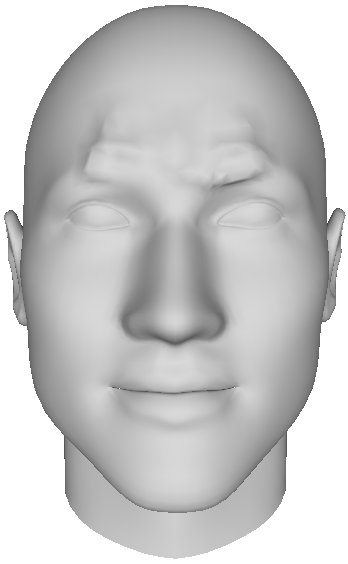
\includegraphics[height=1.8in]{introduction/images/tom_hanks_frontal_awards_facegen_no_texture}\hfill
	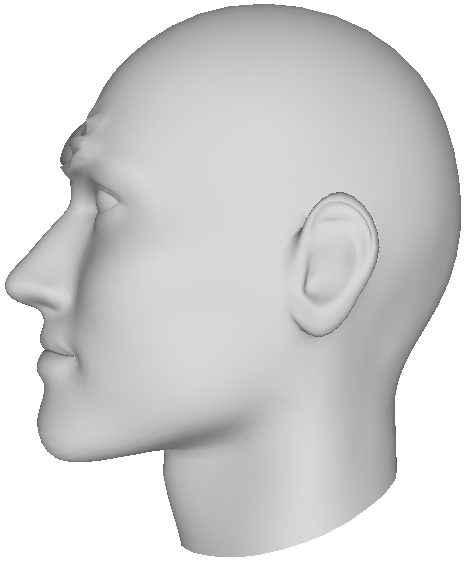
\includegraphics[height=1.8in]{introduction/images/tom_hanks_frontal_awards_facegen_no_texture_profile}
	\hspace*{\fill}
	\caption{An example of facial shape recovery by a 3D Morphable Model, 
	         provided by the commercial FaceGen software~\cite{facegen}. The
	         input image (leftmost) of Tom Hanks was provided and keypoints were
	         manually specified. Notice that the texture provides a strong 
	         likeness to Tom Hanks' face, yet the untextured mesh does not.}
\label{fig:facegen_tom_hanks}
\end{figure}
%%%%%%%%%%%%%%%%%%%%%%%%%%%%%%%%%%%%%%%%
%%%%%%%%%%%%%%%%%%%%%%%%%%%%%%%%%%%%%%%%%%%%%%%%%%%%%%%%%%%%%%%%%%%%%%%%%%%%%%%%
\section{Contributions}\label{sec:intro_contrib}
%%%%%%%%%%%%%%%%%%%%%%%%%%%%%%%%%%%%%%%%%%%%%%%%%%%%%%%%%%%%%%%%%%%%%%%%%%%%%%%%

%%%%%%%%%%%%%%%%%%%%%%%%%%%%%%%%%%%%%%%%%%%%%%%%%%%%%%%%%%%%%%%%%%%%%%%%%%%%%%%%
\section{Publications}\label{sec:intro_pubs}
%%%%%%%%%%%%%%%%%%%%%%%%%%%%%%%%%%%%%%%%%%%%%%%%%%%%%%%%%%%%%%%%%%%%%%%%%%%%%%%%
In this section I provide a list of publication that were authored during the
course of my thesis. These publications are split into two sections, those
that are related to the contents of this thesis 
(\cref{subsec:intro_rel_pubs}) and other publications that 
are not directly relevant (\cref{subsec:intro_other_pubs}).
%%%%%%%%%%%%%%%%%%%%%%%%%%%%%%%%%%%%%%%%%%%%%%%%%%%%%%%%%%%%%%%%%%%%%%%%%%%%%%%%
\subsection{Related Publications}\label{subsec:intro_rel_pubs}
%%%%%%%%%%%%%%%%%%%%%%%%%%%%%%%%%%%%%%%%%%%%%%%%%%%%%%%%%%%%%%%%%%%%%%%%%%%%%%%%
\begin{itemize}
	\item\bibentry{Snape:2014de}
	\item\bibentry{Snape:2015gl}
	\item\bibentry{Snape:2015hj}
\end{itemize}
%%%%%%%%%%%%%%%%%%%%%%%%%%%%%%%%%%%%%%%%%%%%%%%%%%%%%%%%%%%%%%%%%%%%%%%%%%%%%%%%
\subsection{Other Publications}\label{subsec:intro_other_pubs}
%%%%%%%%%%%%%%%%%%%%%%%%%%%%%%%%%%%%%%%%%%%%%%%%%%%%%%%%%%%%%%%%%%%%%%%%%%%%%%%%
\begin{itemize}
	\item\bibentry{menpo14}
	\item\bibentry{Chrysos:2015gt}
\end{itemize}
%%%%%%%%%%%%%%%%%%%%%%%%%%%%%%%%%%%%%%%%%%%%%%%%%%%%%%%%%%%%%%%%%%%%%%%%%%%%%%%%
\section{Outline}\label{sec:introduction_outline}
%%%%%%%%%%%%%%%%%%%%%%%%%%%%%%%%%%%%%%%%%%%%%%%%%%%%%%%%%%%%%%%%%%%%%%%%%%%%%%%%

%%%%%%%%%%%%%%%%%%%%%%%%%%%%%%%%%%%%%%%%%%%%%%%%%%%%%%%%%%%%%%%%%%%%%%%%%%%%%%%%